\section{Grammar}
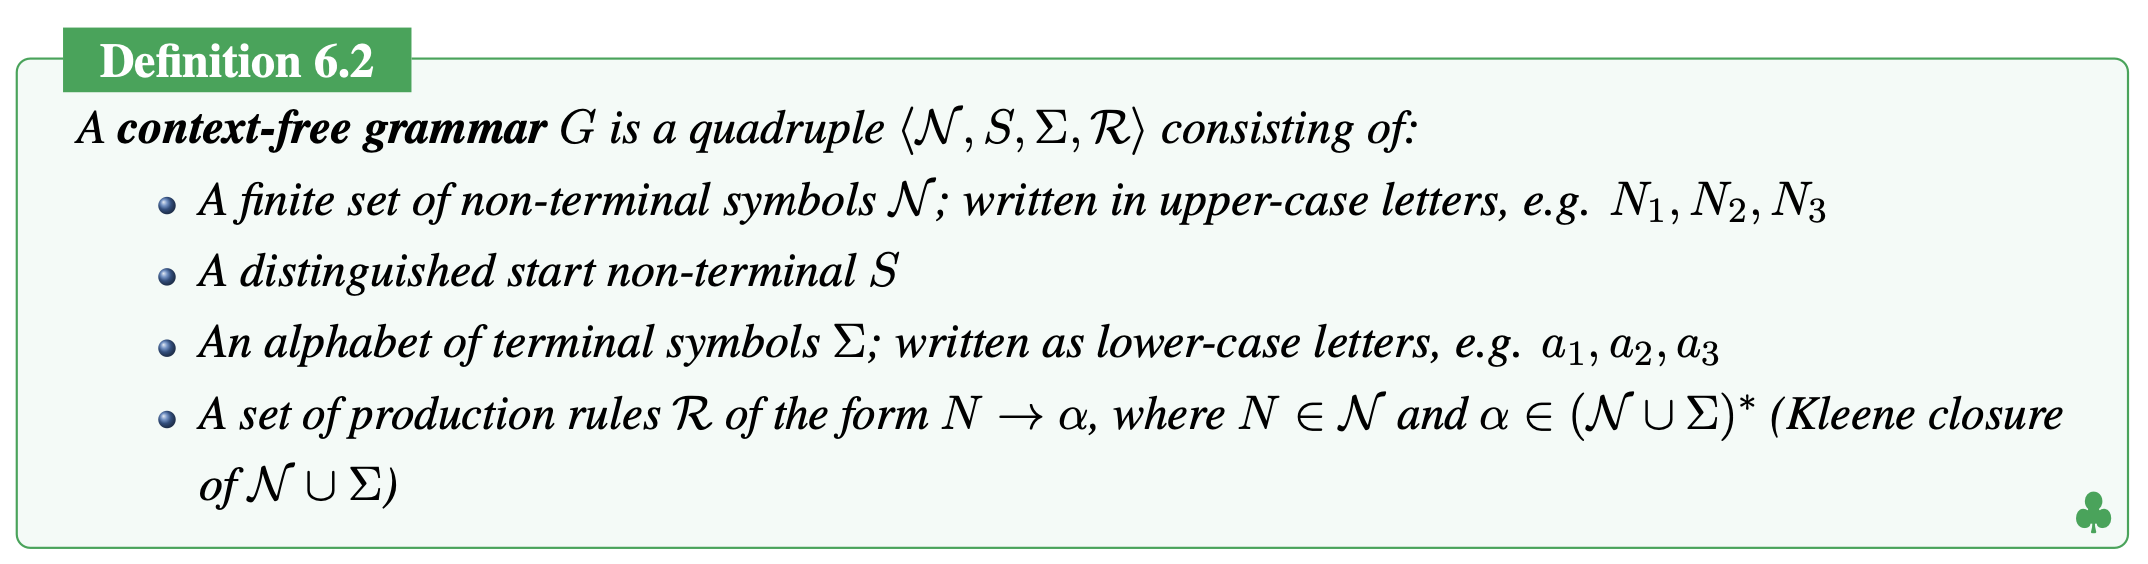
\includegraphics[width=7cm]{cfg_def.png}
\subsection{Chomsky Normal Form}
Grammar is in Chomsky Normal Form (CNF) if RHS of every production rule includes either two non-terminals or a single terminal symbol:
$N_1 \rightarrow N_2 N_3$ or $N \rightarrow a$\\
\subsection{PCFG}
Probabilistic Context Free Grammar (PCFG) $\langle \mathcal{N}, S, \sum, \mathcal{R}, \mathcal{P} \rangle$, where $\mathcal{P}$ are probabilities assigned to each production rule.\\
\subsection{WCFG}
Weighted Context Free Grammar (WCFG) $\langle \mathcal{N}, S, \sum, \mathcal{R}, \mathcal{W} \rangle$, where $\mathcal{W}$ are non-negative weights assigned to each production rule. PCFG is special case of WCFG.